\documentclass{beamer}

\usepackage{geometry} % Pour passer au format A4
\usepackage{graphicx} % Required for including pictures
\usepackage{float} % 

\usepackage{amsmath,amsfonts,amssymb,amsthm}
\usepackage[T1]{fontenc} 
\usepackage[english,francais]{babel}
\usepackage[utf8]{inputenc}
\usepackage{lmodern}

\usetheme{Warsaw}

\title{Angles et parallélisme}

\begin{document}

\frame{\titlepage}

%-----------------------------------111111111111111111111111111111111111
\section{Angles}
%----------------------------------------------------------------------


\frame{\tableofcontents[sectionstyle=show/shaded, subsectionstyle=show/shaded]}

\begin{frame}
  \frametitle{Angles adjacents}

  \begin{alertblock}{Définition :}	
    Deux angles sont adjacents si :
    \begin{itemize}
    \item Ils ont un même sommet;
    \item Ils ont un côté commun;
    \item Ils sont situés de part et d'autre de ce côté commun.
    \end{itemize}
  \end{alertblock}

  \begin{figure}[H]
    \centering
    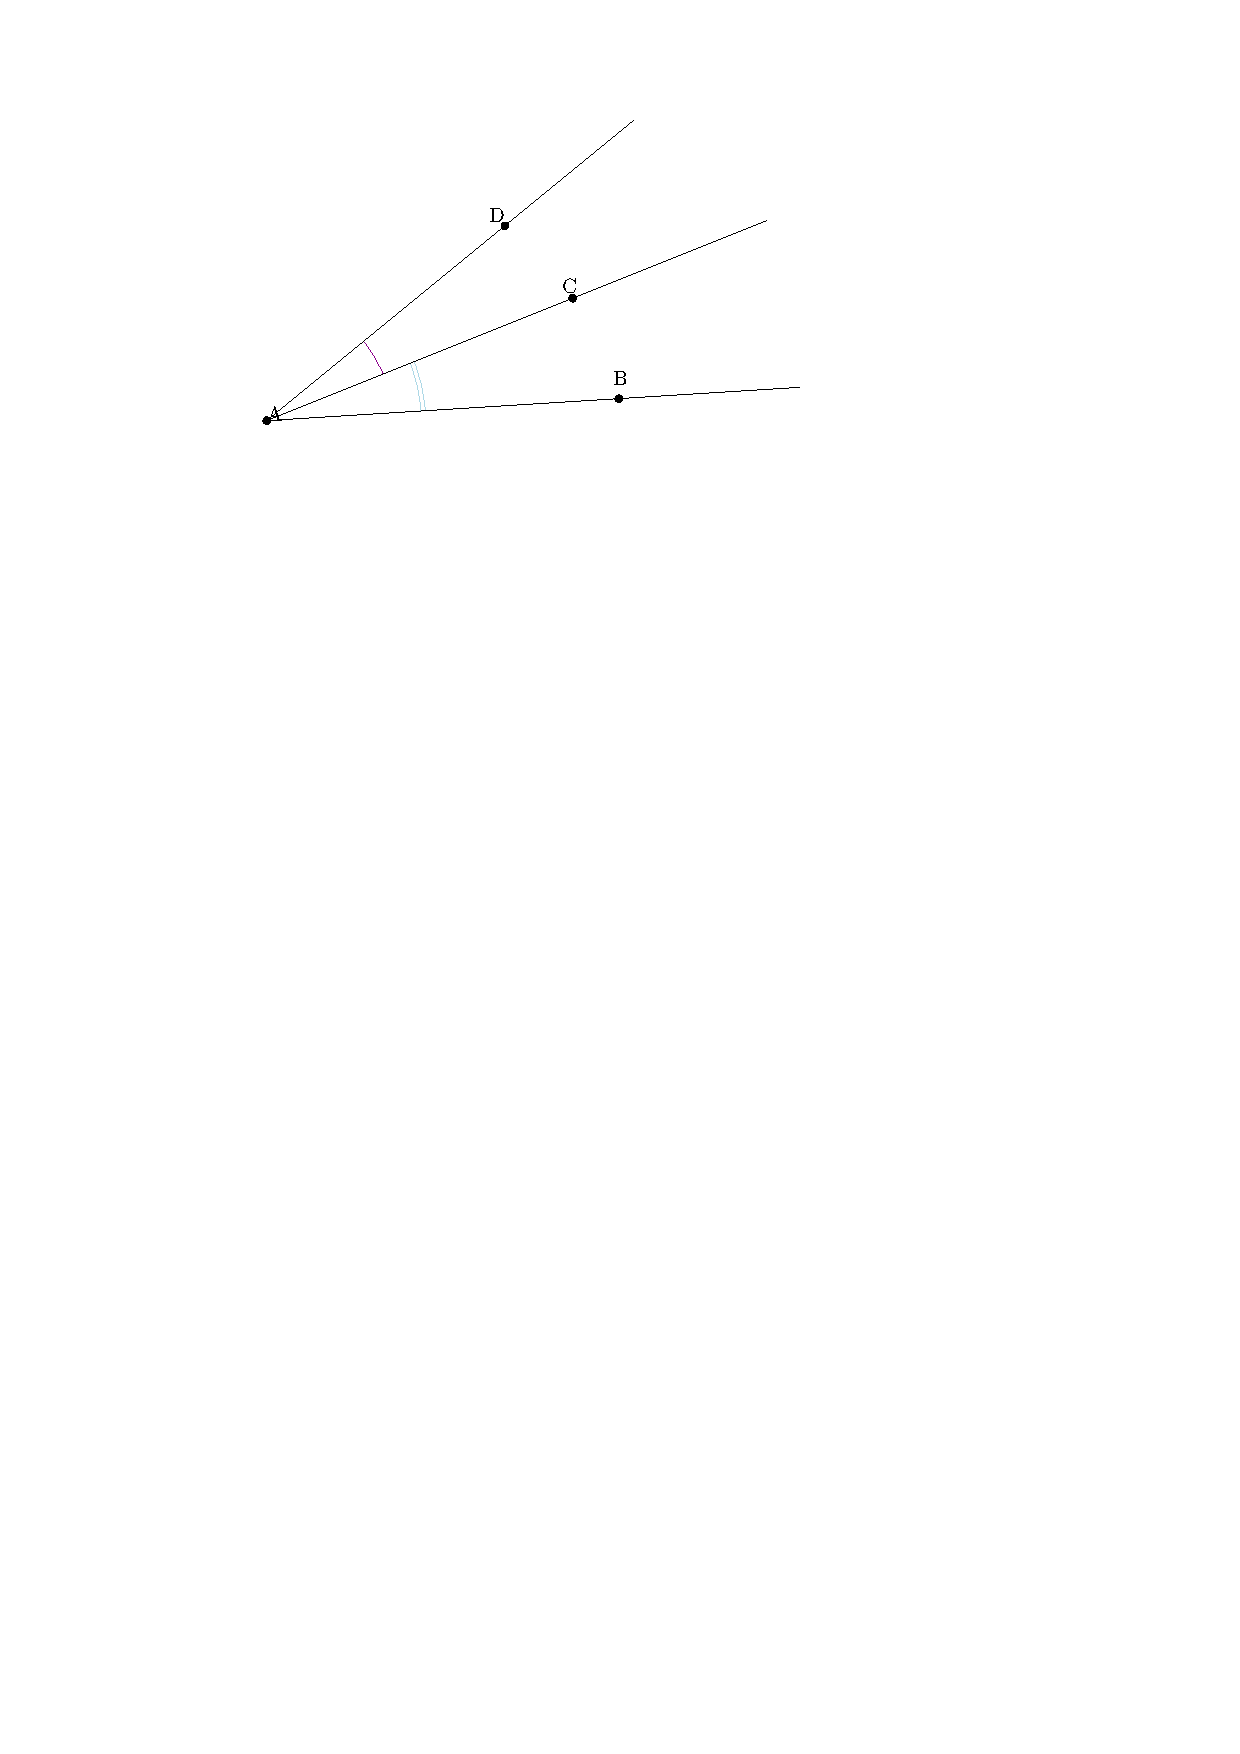
\includegraphics[width=0.4\linewidth]{5x10-angles/sources/adjacents.pdf}
    \\$\widehat{BAC}$ et $\widehat{DAC}$ sont adjacents.
  \end{figure}

\end{frame}

\begin{frame}
  \frametitle{Angles opposés par le sommet}
  \begin{alertblock}{Définition :}	
    Deux angles sont opposés par le sommet si :
    \begin{itemize}
    \item Ils ont un même sommet;
    \item Les côtés de l'un sont le prolongement des côtés de l'autre.
    \end{itemize}
  \end{alertblock}
  \begin{columns}[t]
    \begin{column}{5cm}
      \begin{figure}[H]
        \centering
        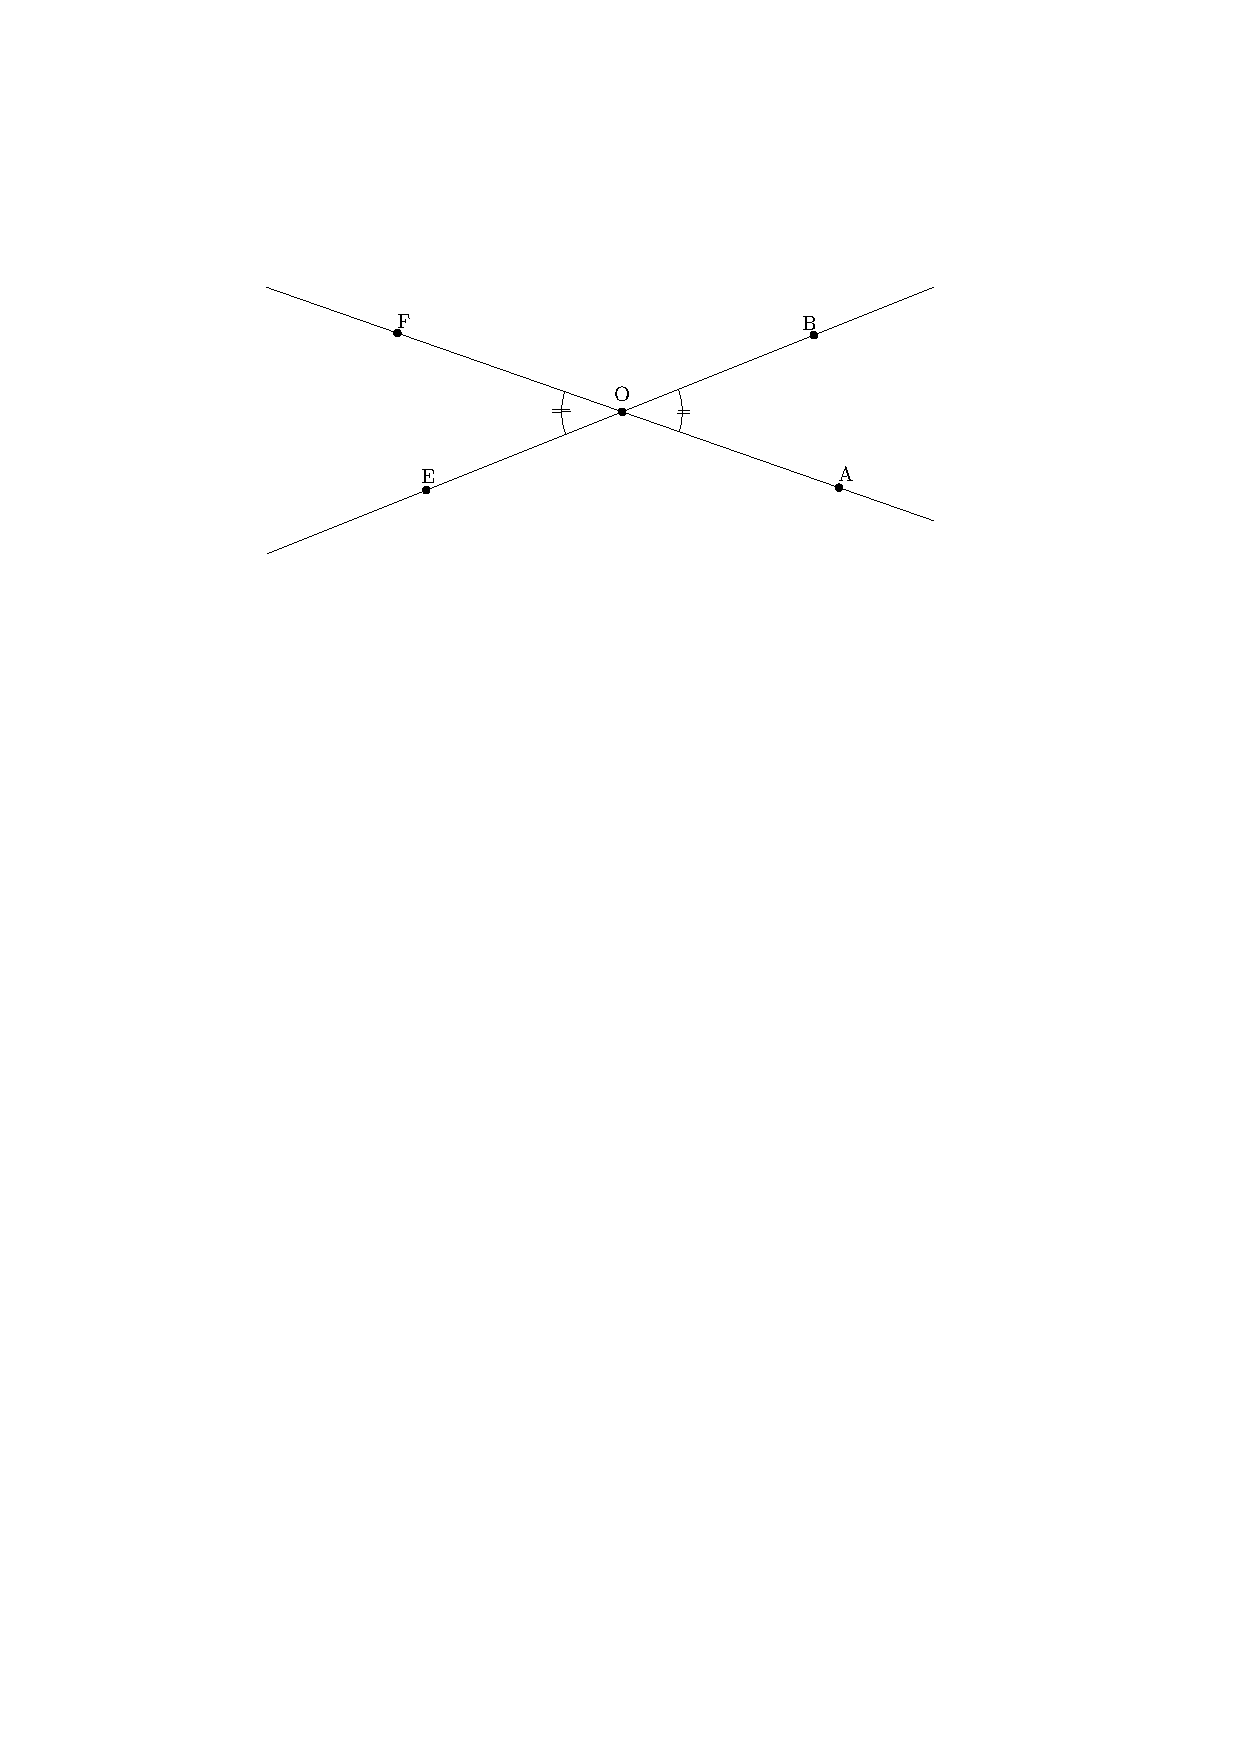
\includegraphics[width=\linewidth]{5x10-angles/sources/opposes.pdf}
        \\$\widehat{EOF}$ et $\widehat{BOA}$ sont opposés par le sommet.    
      \end{figure} 
    \end{column}
    \begin{column}{5cm}
      \begin{block}{Propriété}
        Deux angles opposés par le sommet sont égaux.     
      \end{block}
      $$\widehat{EOF} = \widehat{BOA}$$ 
    \end{column}
  \end{columns} 
\end{frame}

\begin{frame}
  \frametitle{Angles complémentaires}
  \begin{alertblock}{Définition :}	
    Deux angles sont complémentaires si la somme de leurs mesures est égale à 90\char6.
  \end{alertblock}
  \begin{columns}[t]
    \begin{column}{5cm}
      \begin{figure}[H]
        \centering
        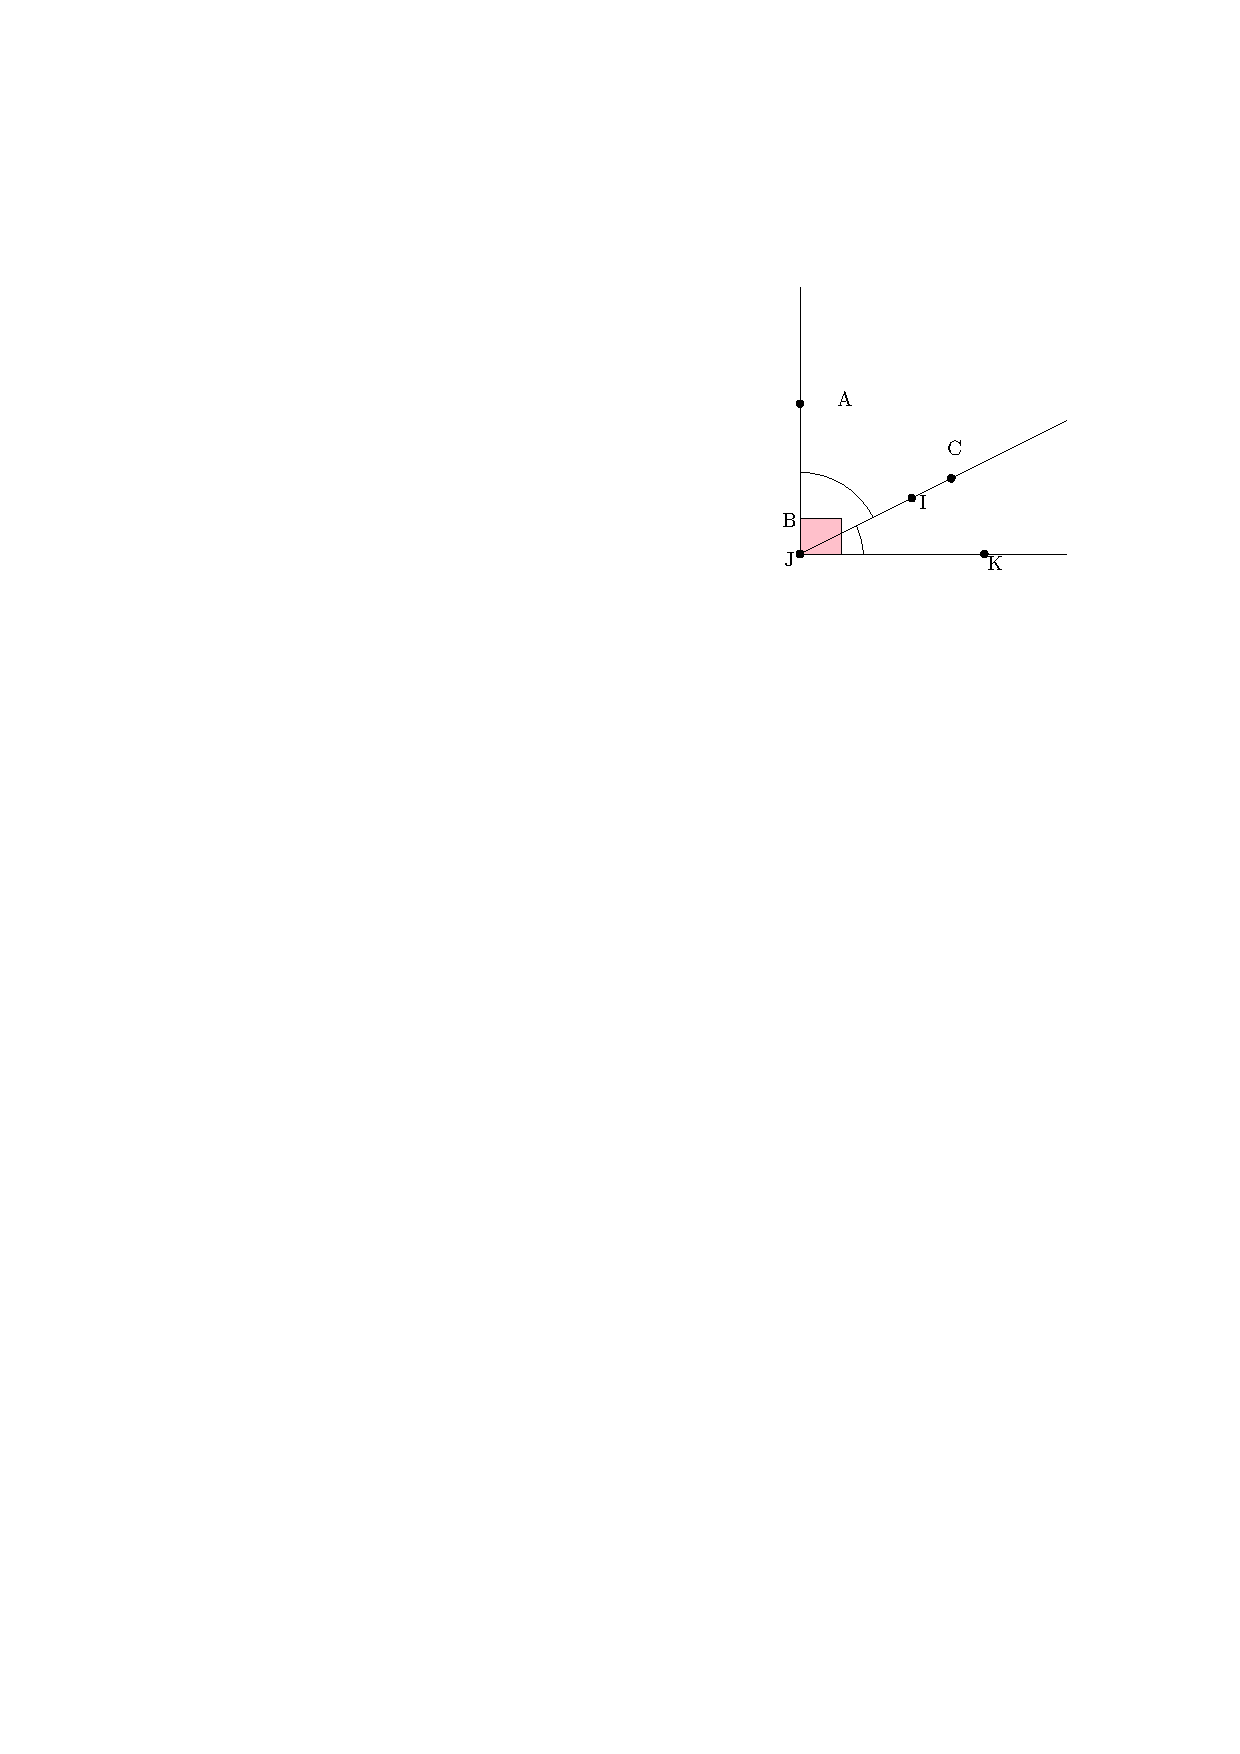
\includegraphics[width=0.8\linewidth]{5x10-angles/sources/complementaires.pdf}
      \end{figure}
    \end{column}
    \begin{column}{5cm}
      \vspace{1cm}\\
      $\widehat{ABC}$ et $\widehat{IJK}$ sont complémentaires.  
    \end{column}
  \end{columns}    
\end{frame}

\begin{frame}
  \frametitle{Angles supplémenaitres}
  \begin{alertblock}{Définition :}	
    Deux angles sont supplémentaires si la somme de leurs mesures est égale à 180\char6.
  \end{alertblock}
  \begin{columns}[t]
    \begin{column}{5cm}
      \begin{figure}[H]
        \centering
        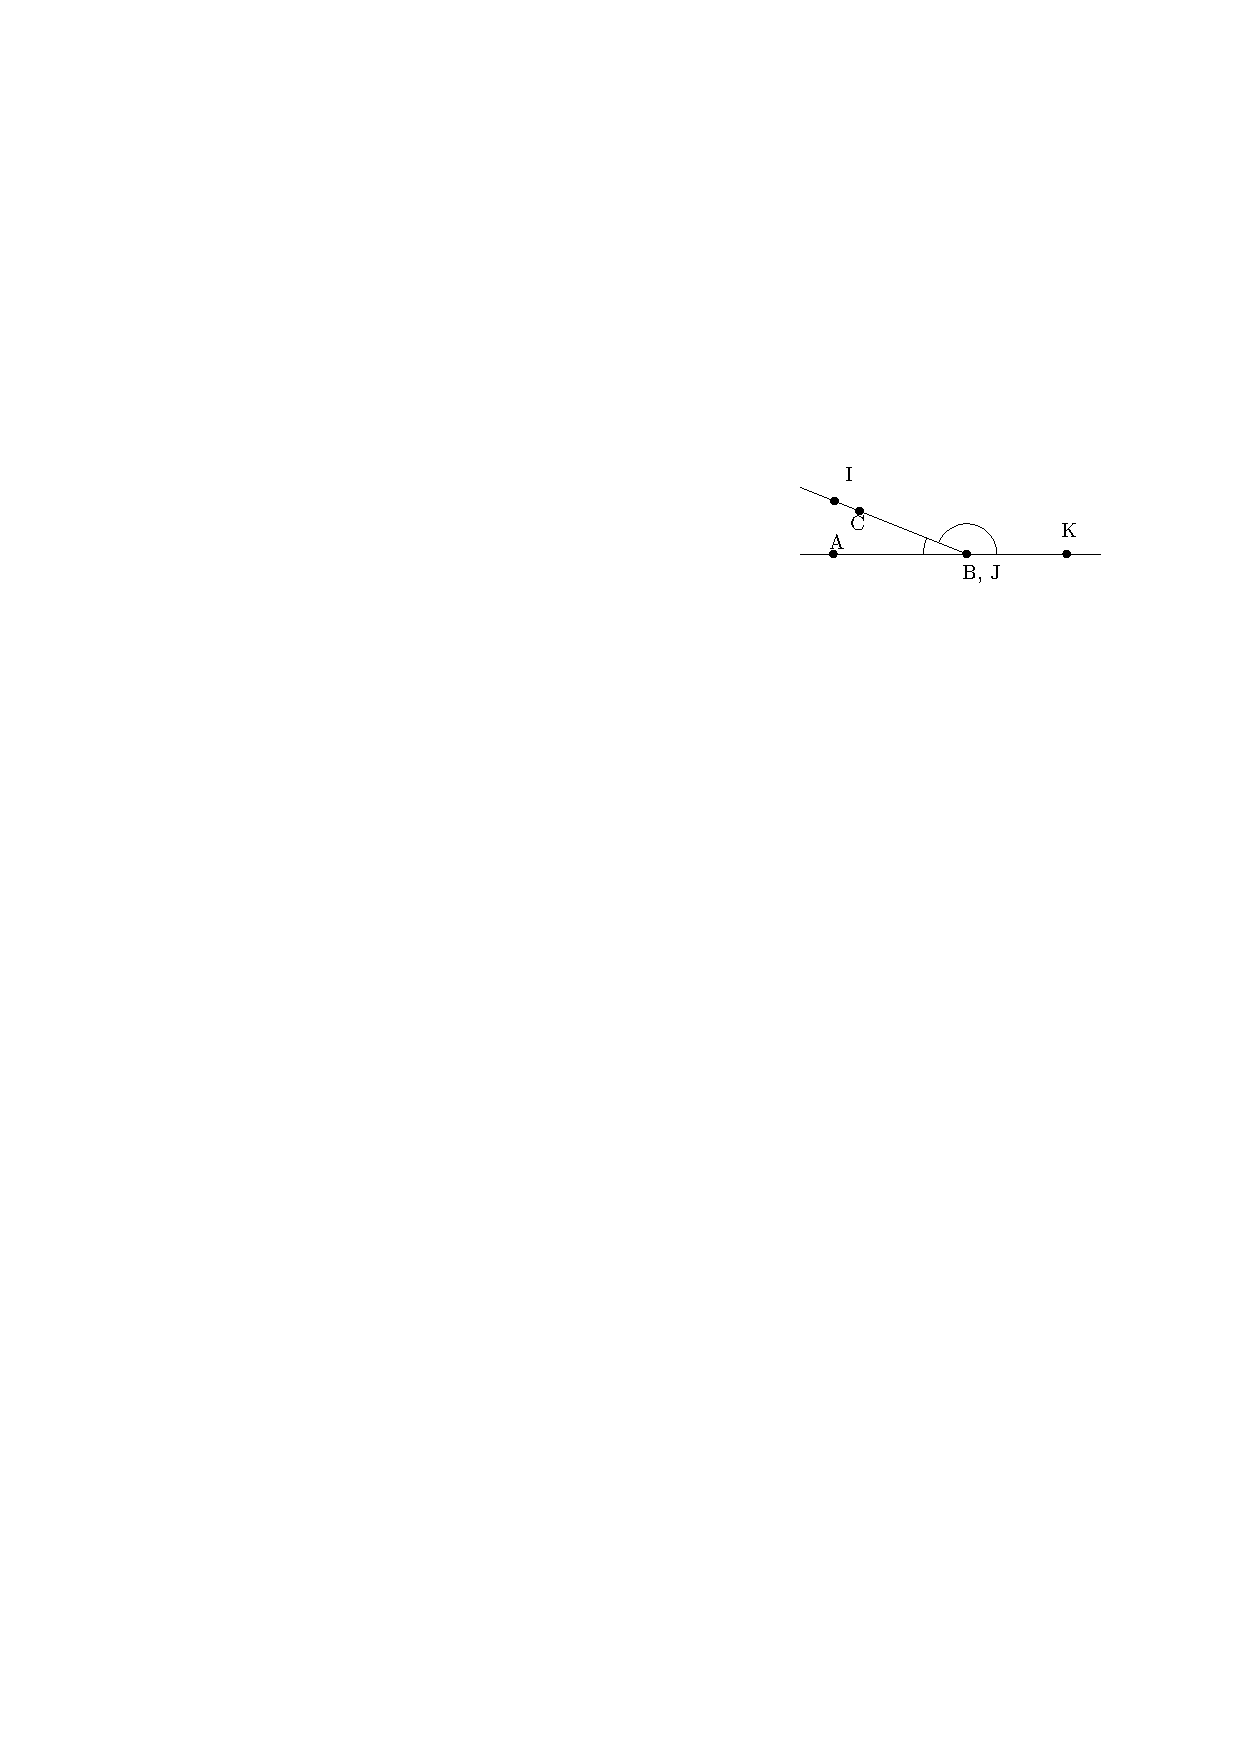
\includegraphics[width=\linewidth]{5x10-angles/sources/supplementaires.pdf}
      \end{figure}
    \end{column}
    \begin{column}{5cm}
      \vspace{1cm}\\
      $\widehat{ABC}$ et $\widehat{IJK}$ sont supplémenaitres.  
    \end{column}
  \end{columns}    
\end{frame}

%-----------------------------------111111111111111111111111111111111111
\section{Parallélisme}
%----------------------------------------------------------------------

\frame{\tableofcontents[sectionstyle=show/shaded, subsectionstyle=show/shaded]}

\begin{frame}
  \frametitle{Angles alternes-internes}
  Soient deux droites $d_1$ et $d_2$ coupées par une troisième droite $d_3$.
  \begin{columns}[t]
    \begin{column}{5cm}
      \begin{figure}[H]
        \centering
        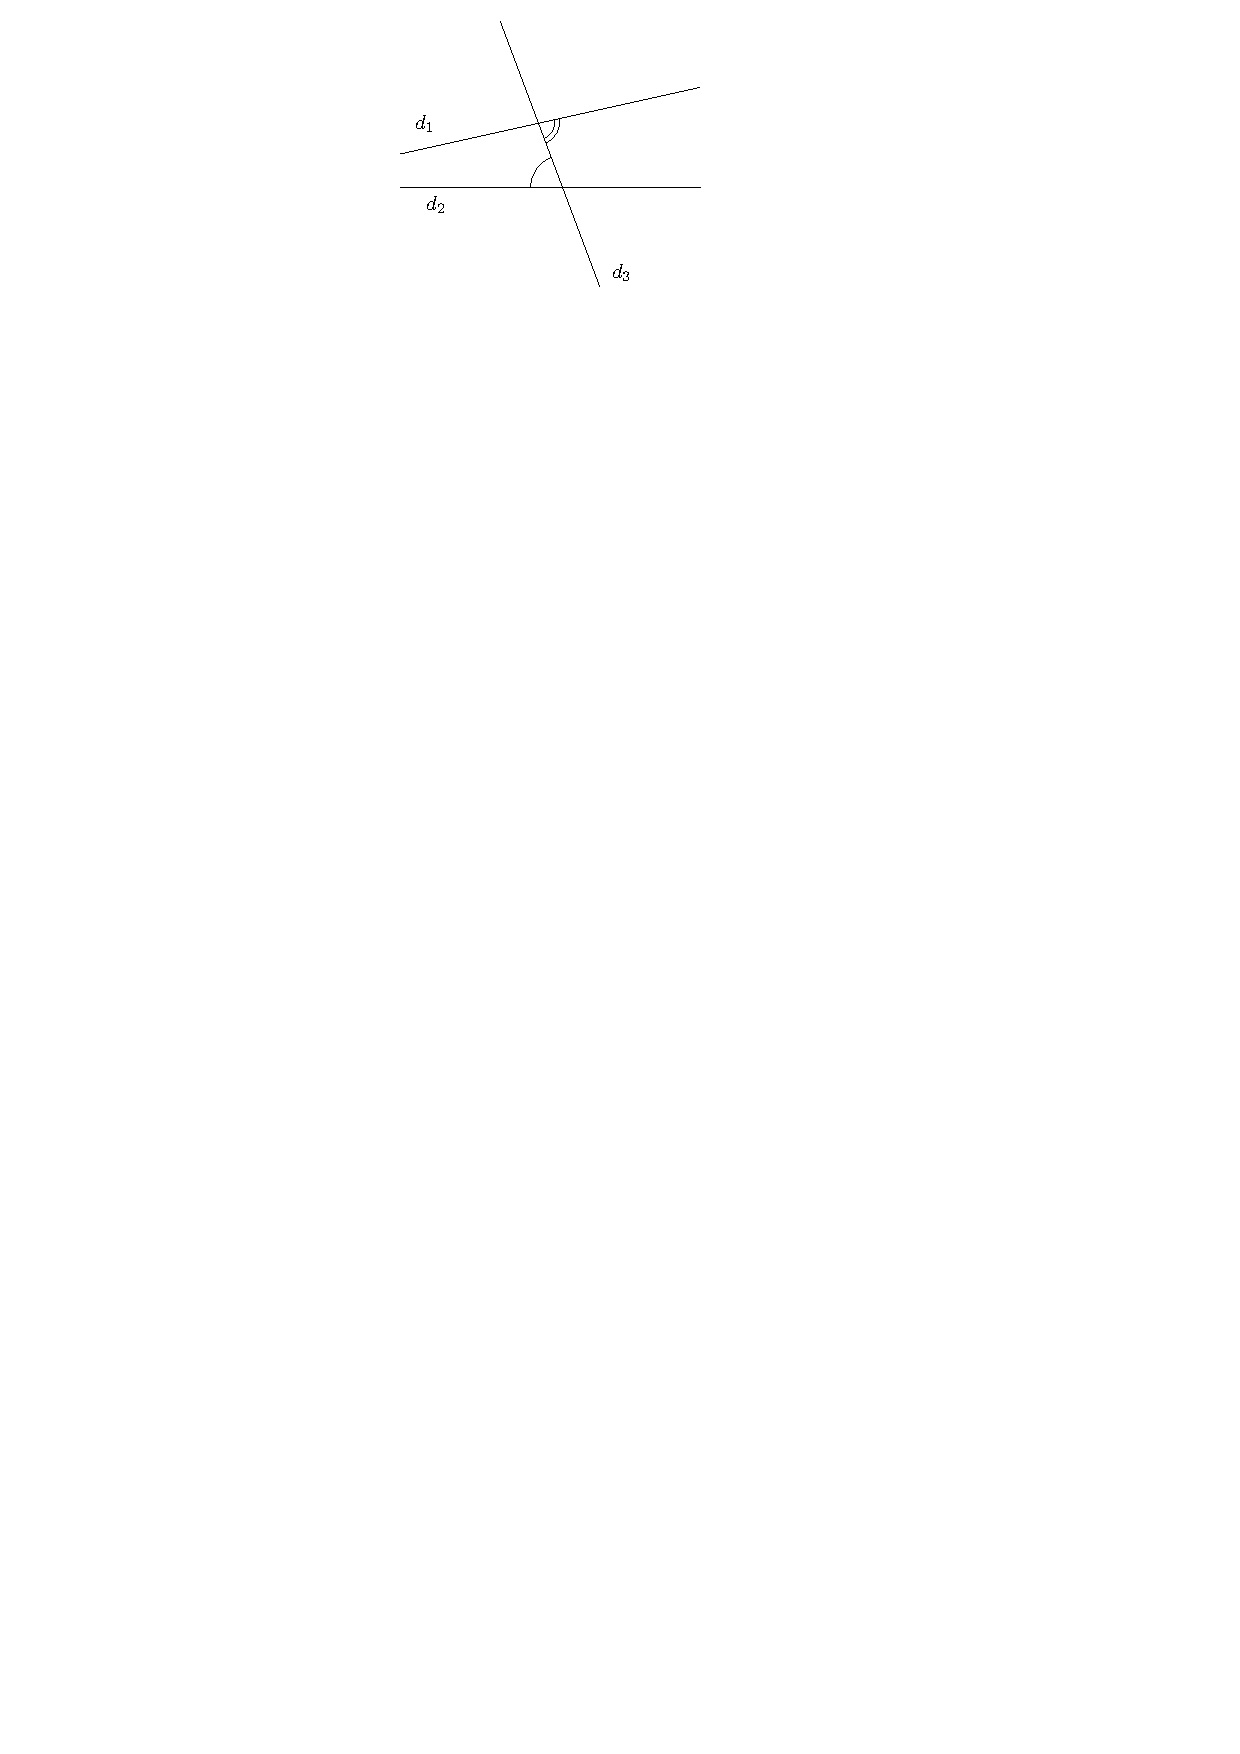
\includegraphics[width=0.6\linewidth]{5x10-angles/sources/ai-1.pdf}
      \end{figure}
      \begin{block}{Définition :}	
        Angles alternes-internes.
      \end{block}   

    \end{column}
    \begin{column}{5cm}
      \begin{figure}[H]
        \centering
        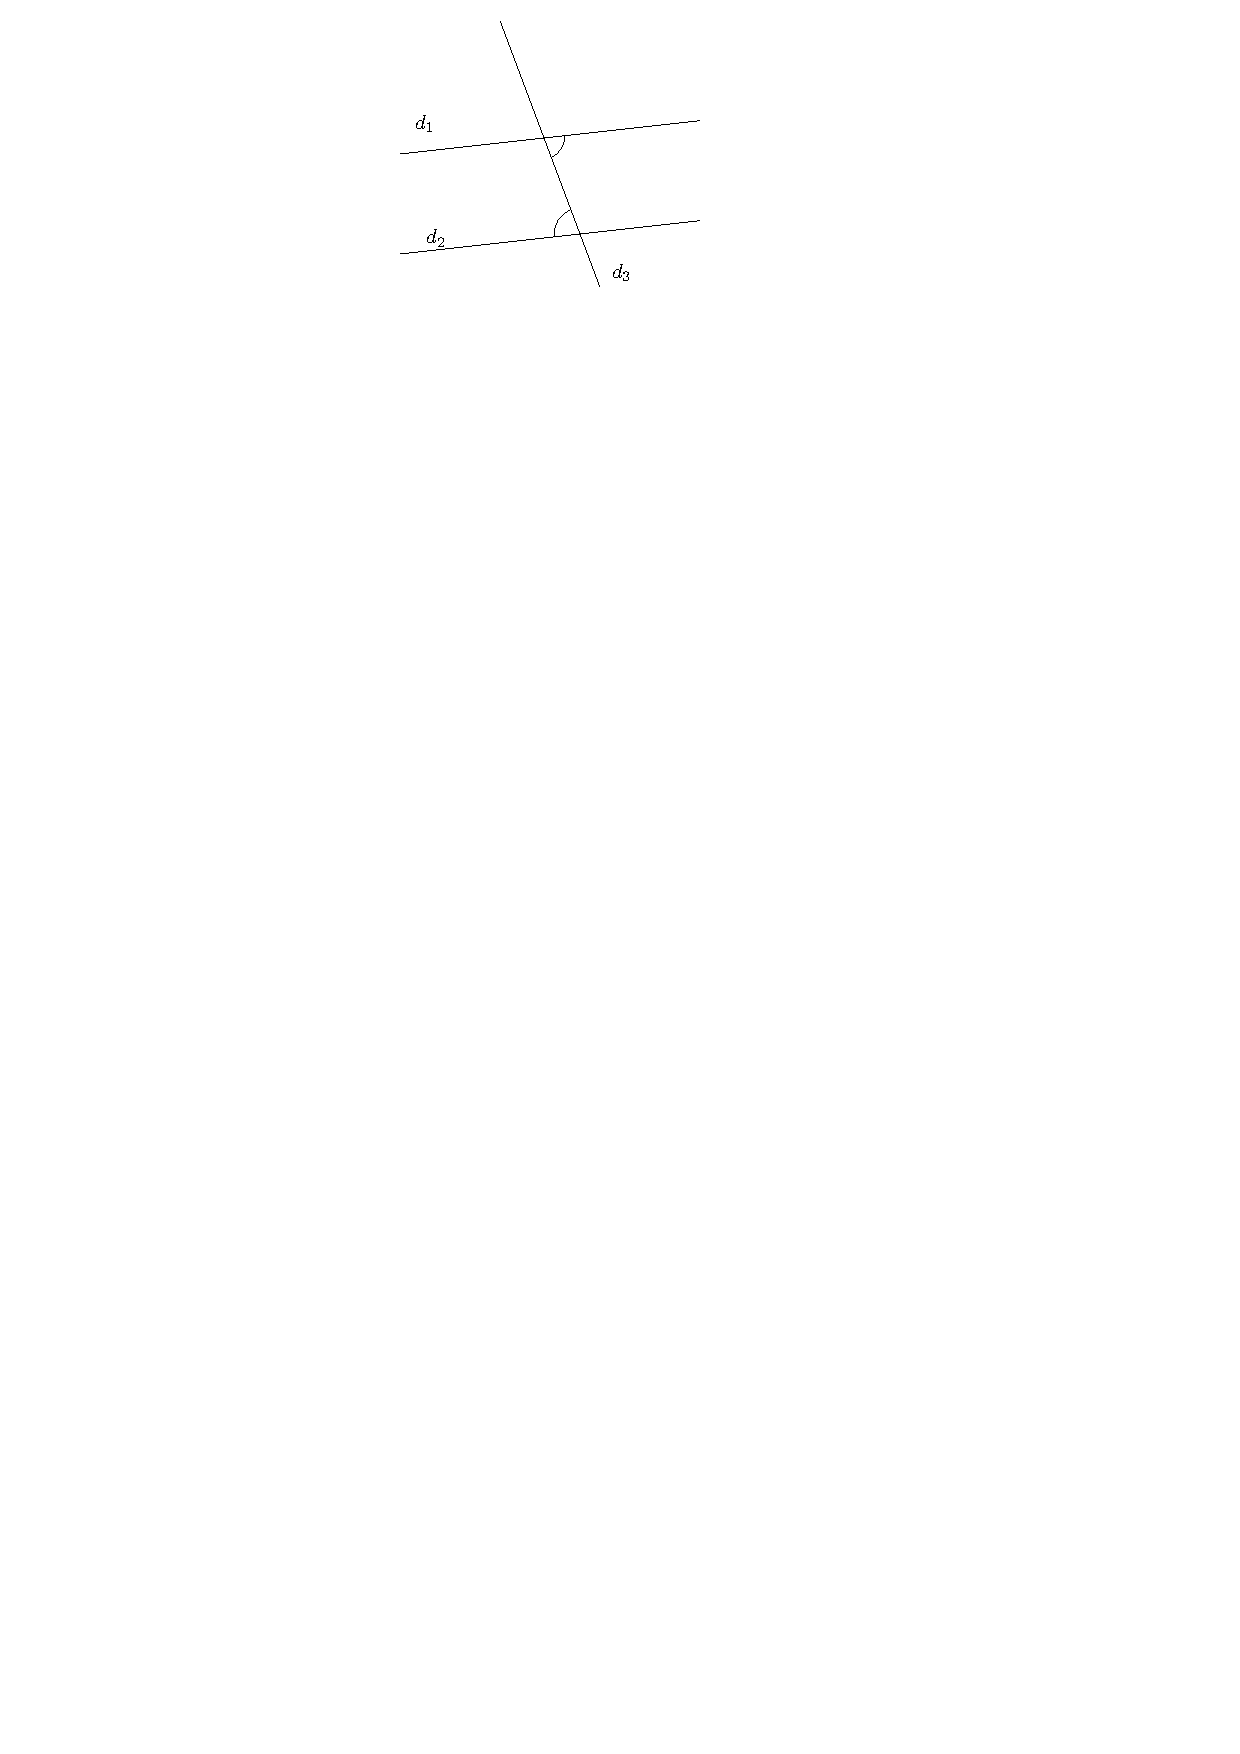
\includegraphics[width=0.6\linewidth]{5x10-angles/sources/ai-2.pdf}
      \end{figure}
      \begin{block}{Propriété :}	
        Si $d_1$ et $d_2$ sont \alert{parallèles}.\\
        Les angles alternes-internes sont \alert{égaux}.
      \end{block}   
    \end{column}
  \end{columns}    
\end{frame}

\begin{frame}
  \frametitle{Angles acorrespondants}
  Soient deux droites $d_1$ et $d_2$ coupées par une troisième droite $d_3$.
  \begin{columns}[t]
    \begin{column}{5cm}
      \begin{figure}[H]
        \centering
        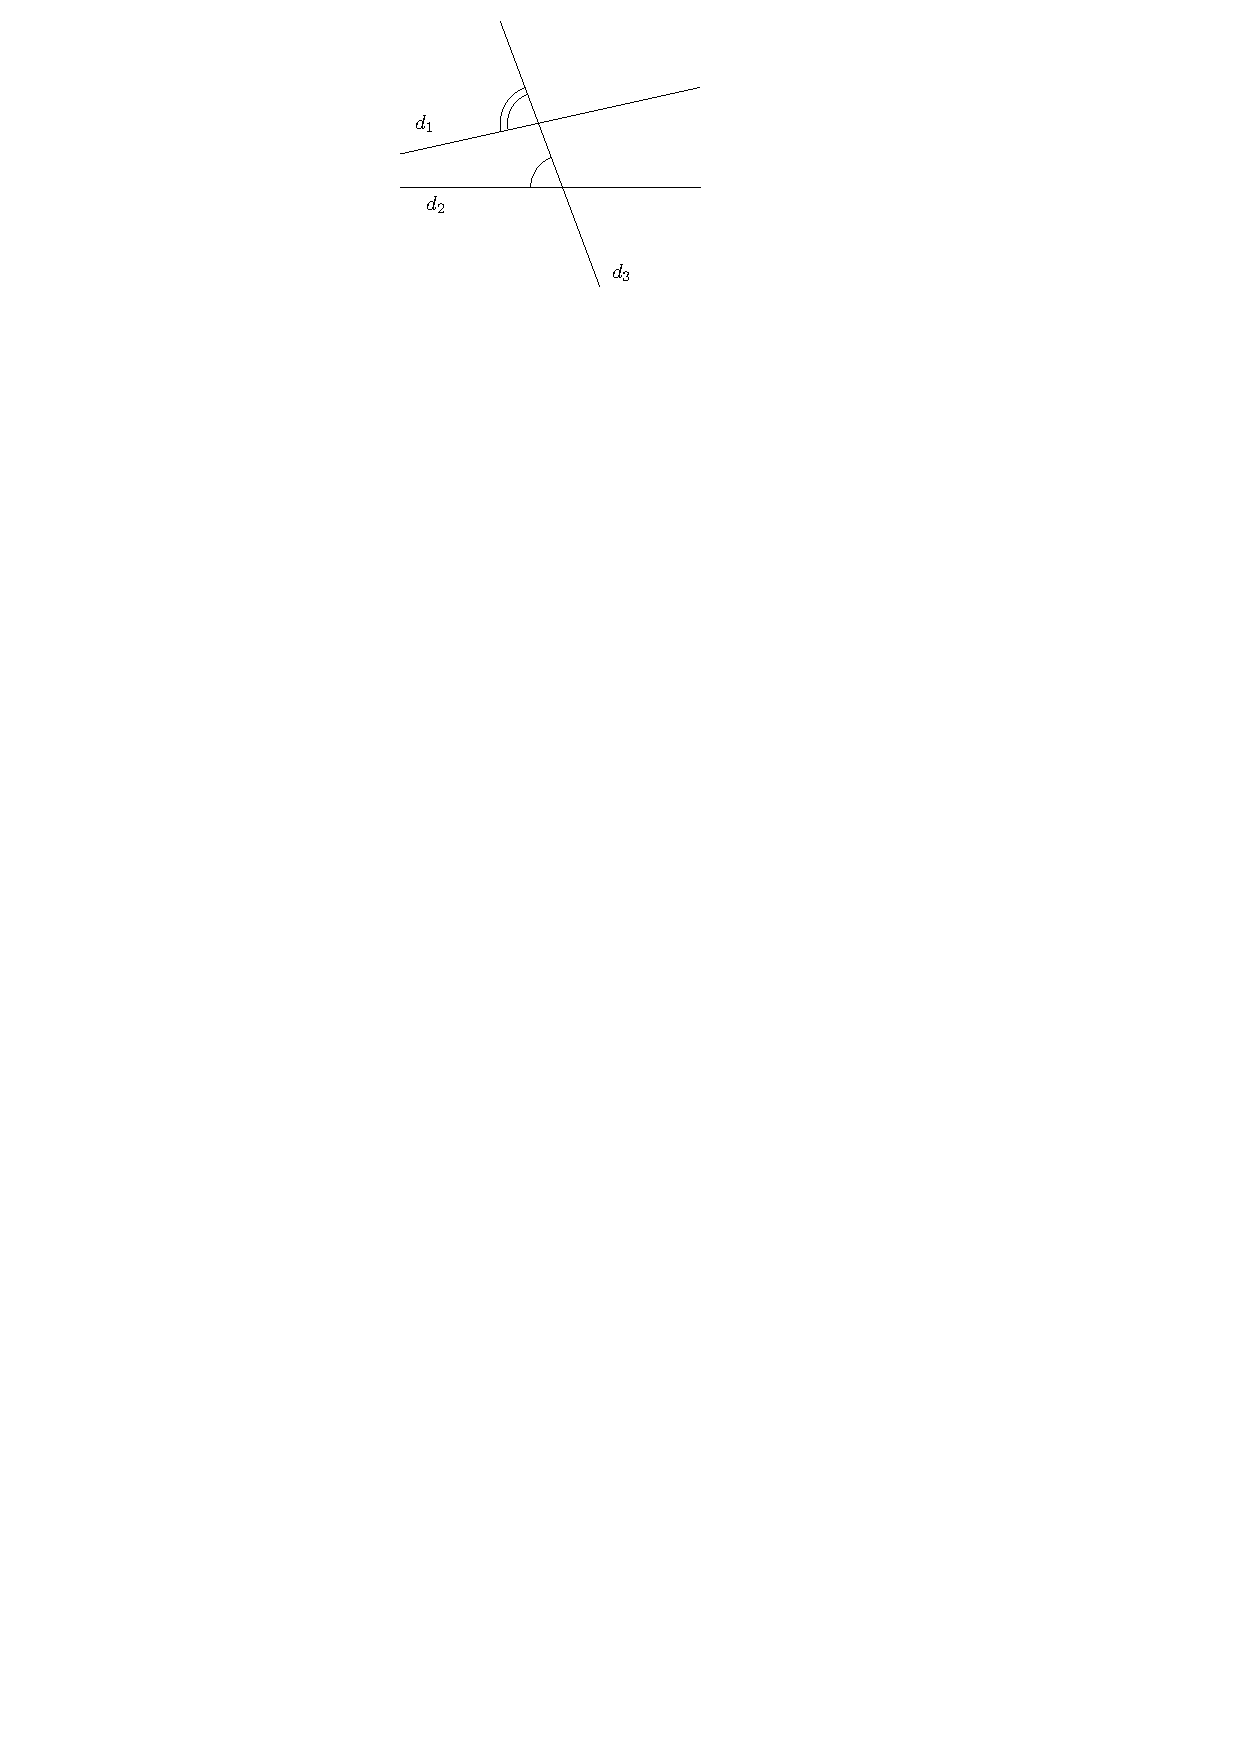
\includegraphics[width=0.6\linewidth]{5x10-angles/sources/corres-1.pdf}
      \end{figure}
      \begin{block}{Définition :}	
        Angles correspondants.
      \end{block}   

    \end{column}
    \begin{column}{5cm}
      \begin{figure}[H]
        \centering
        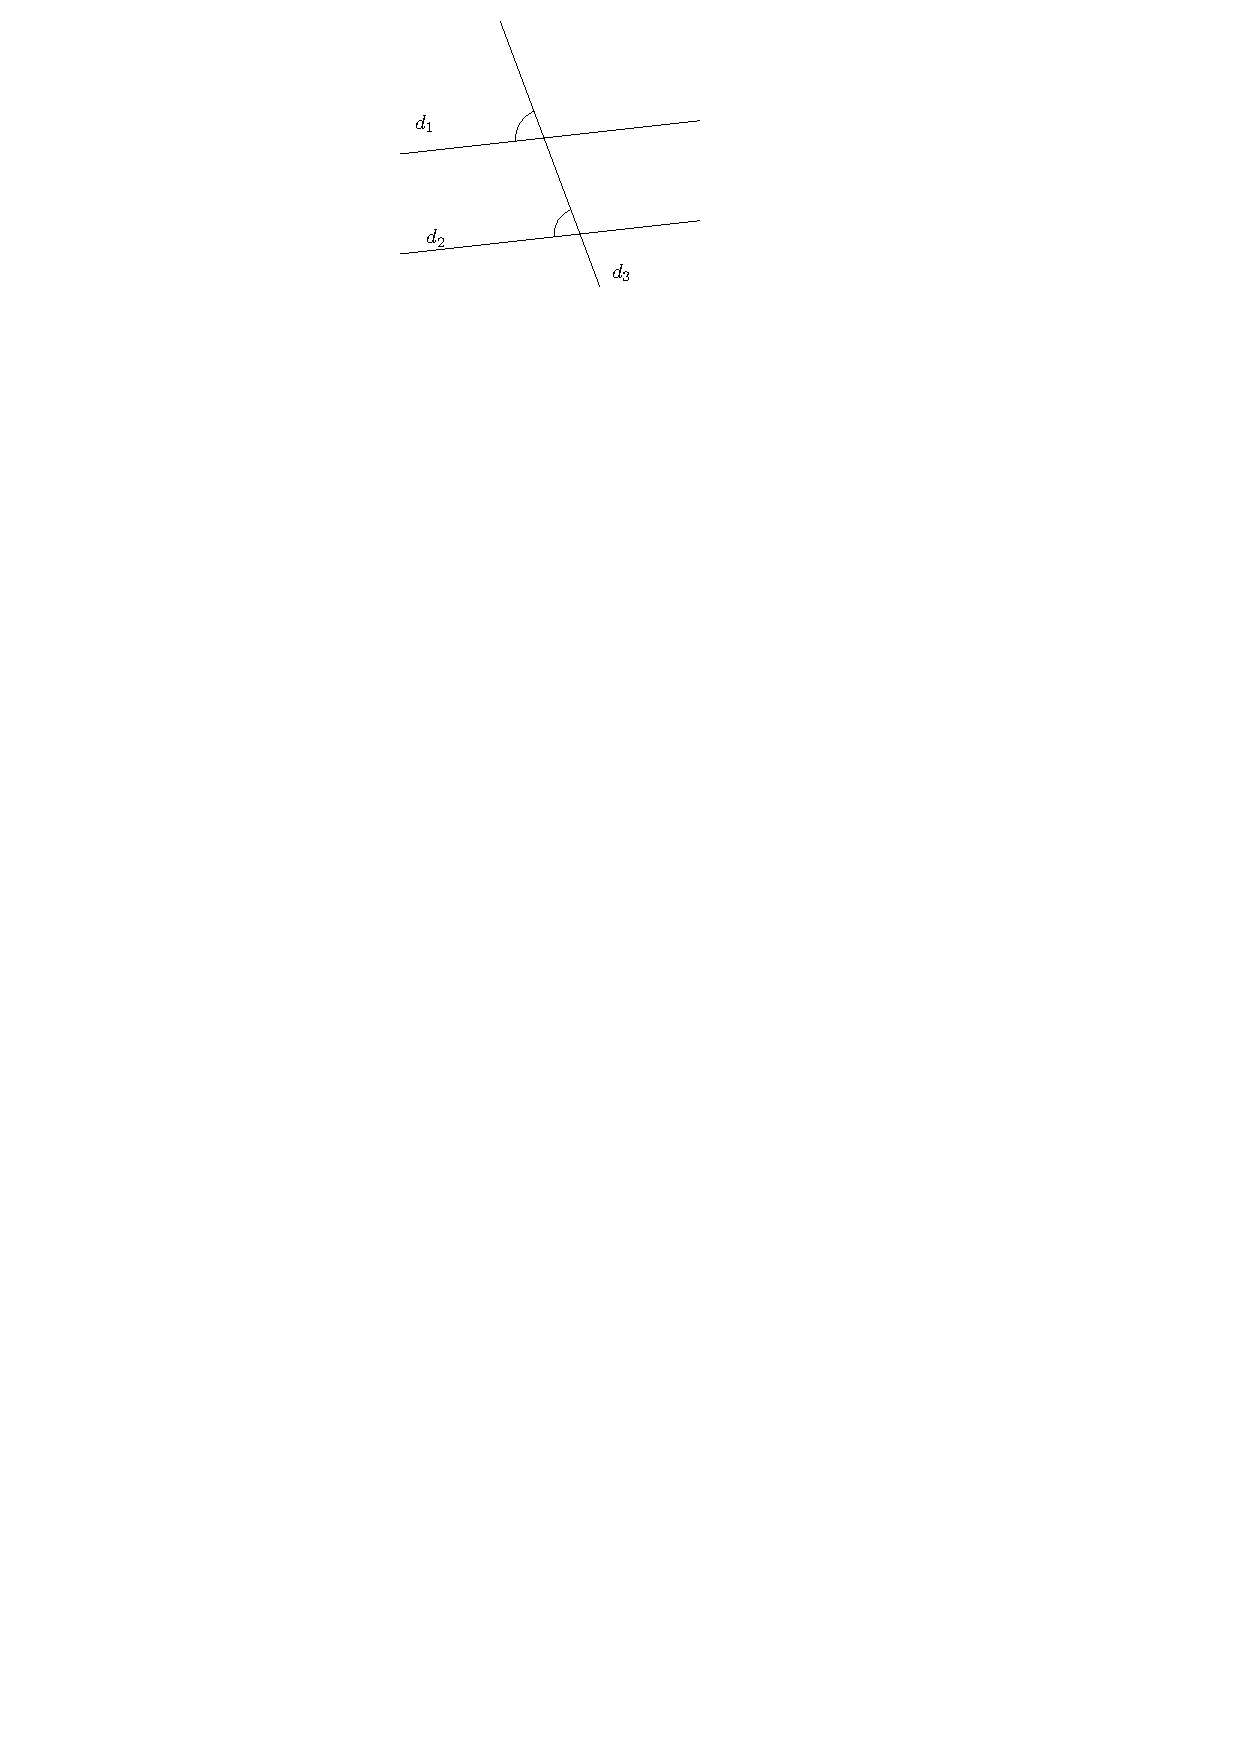
\includegraphics[width=0.6\linewidth]{5x10-angles/sources/corres-2.pdf}
      \end{figure}
      \begin{block}{Propriété :}	
        Si $d_1$ et $d_2$ sont \alert{parallèles}.\\
        Les angles correspondants sont \alert{égaux}.
      \end{block}   
    \end{column}
  \end{columns}    
\end{frame}

\end{document}
